\begin{figure}[ht]
\ffigbox
	{\begin{subfigure}[b]{0.48\linewidth}
		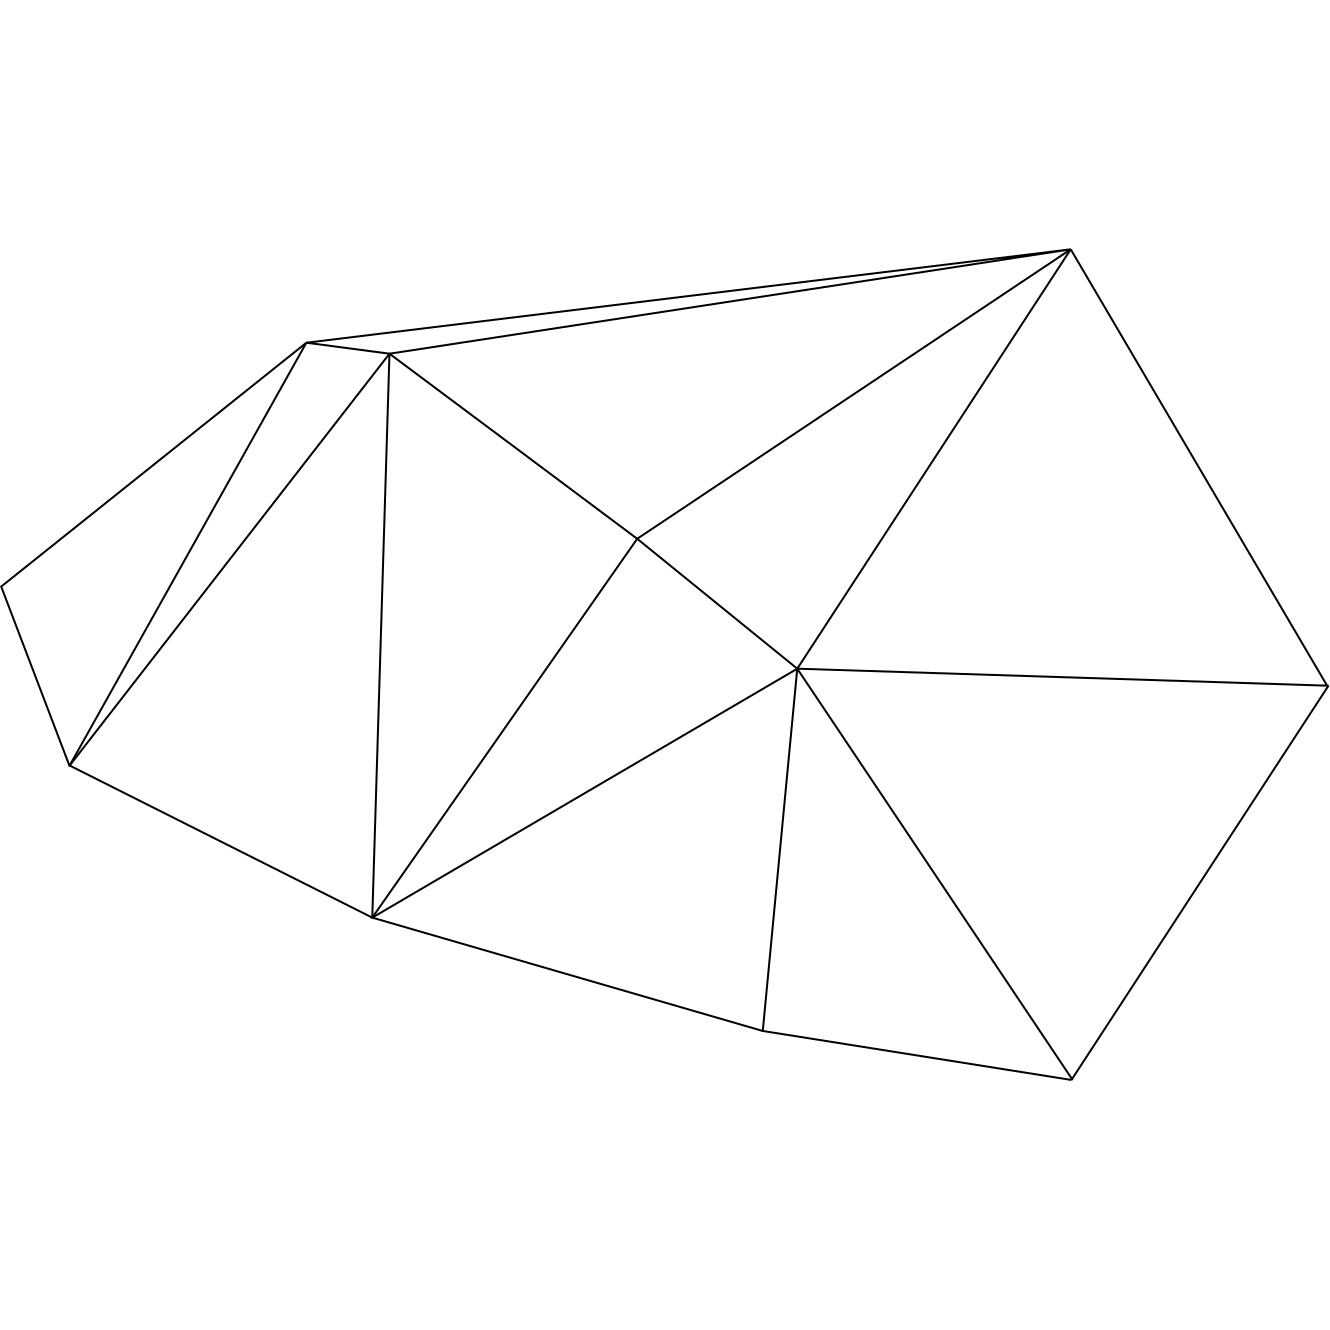
\includegraphics[width=1.0\linewidth,height=0.3\textheight,keepaspectratio]{data/synthetic_meshes/random_circle_tessellation_Dirac_delta_1_v11_f12_wireframe.png}
		\caption{R.Circ v11\_f12 wireframe}\label{fig:rcirc.a}
	\end{subfigure}
	\begin{subfigure}[b]{0.48\linewidth}
		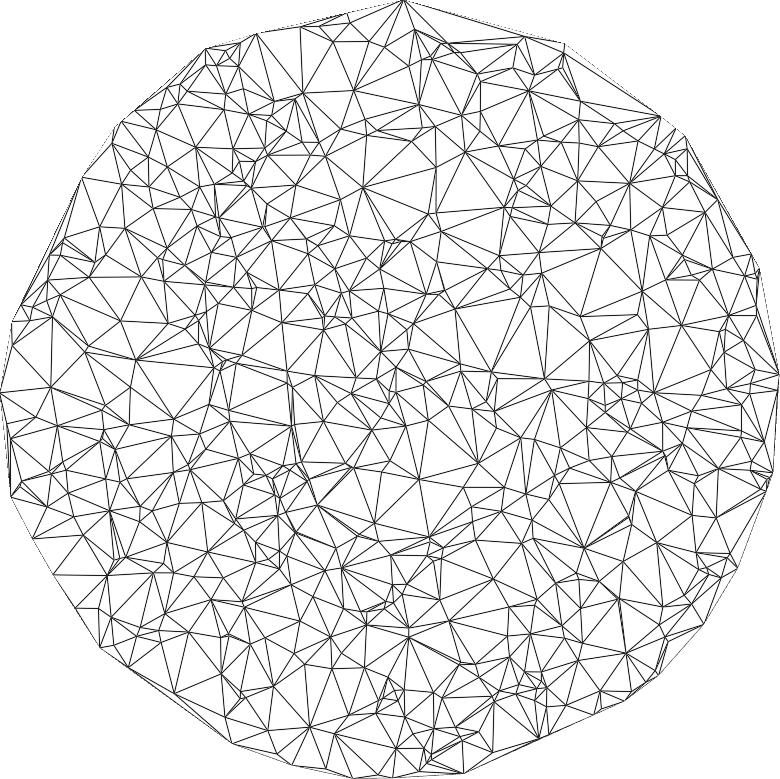
\includegraphics[width=1.0\linewidth,height=0.3\textheight,keepaspectratio]{data/synthetic_meshes/random_circle_tessellation_Dirac_delta_10_v641_f1252_wireframe.png}
		\caption{R.Circ v641\_f1252 wireframe}\label{fig:rcirc.b}
	\end{subfigure}

	\bigskip
	\begin{subfigure}[b]{0.48\linewidth}
		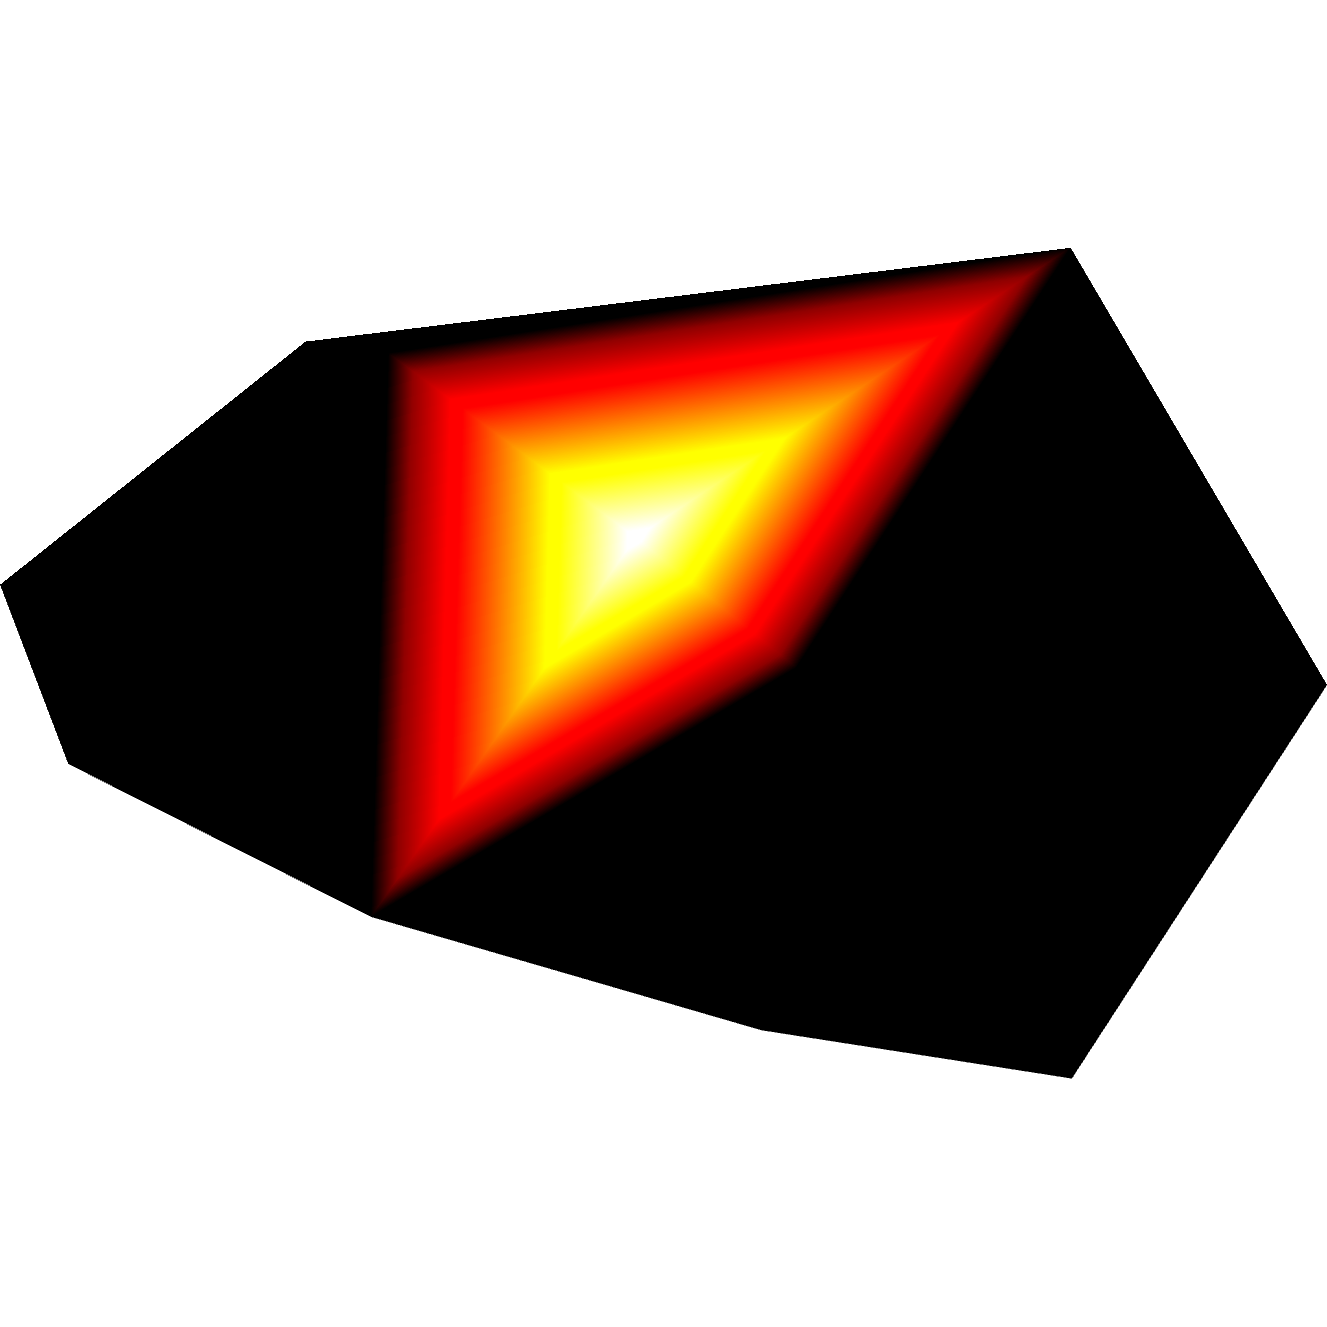
\includegraphics[width=1.0\linewidth,height=0.3\textheight,keepaspectratio]{data/synthetic_meshes/random_circle_tessellation_Dirac_delta_1_v11_f12_funcvals_0iter.png}
		\caption{R.Circ v11\_f12 iter 0}\label{fig:rcirc.c}
	\end{subfigure}
	\begin{subfigure}[b]{0.48\linewidth}
		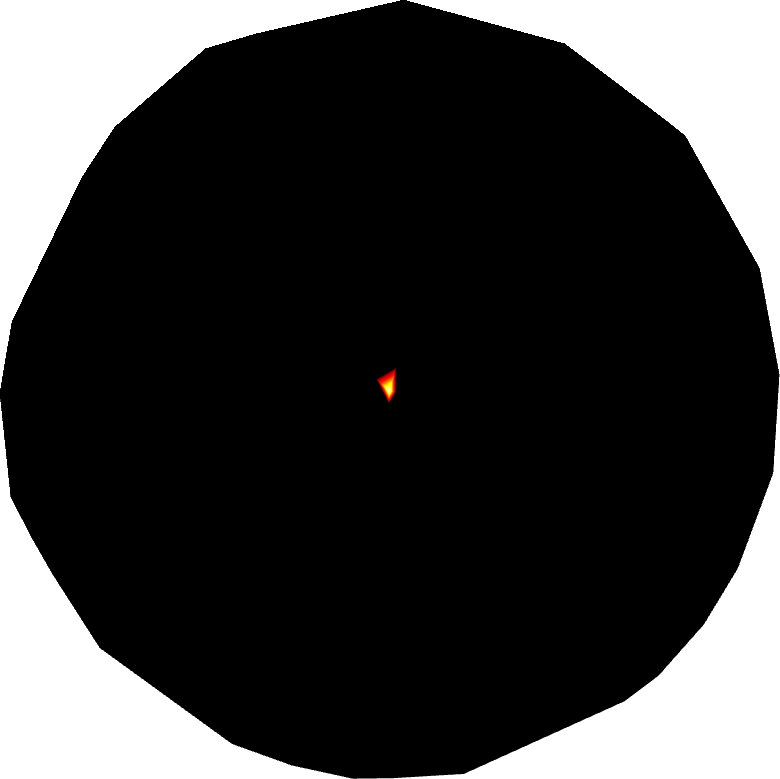
\includegraphics[width=1.0\linewidth,height=0.3\textheight,keepaspectratio]{data/synthetic_meshes/random_circle_tessellation_Dirac_delta_10_v641_f1252_funcvals_0iter.png}
		\caption{R.Circ v641\_f1252 iter 0}\label{fig:rcirc.d}
	\end{subfigure}

	\bigskip
	\begin{subfigure}[b]{0.48\linewidth}
		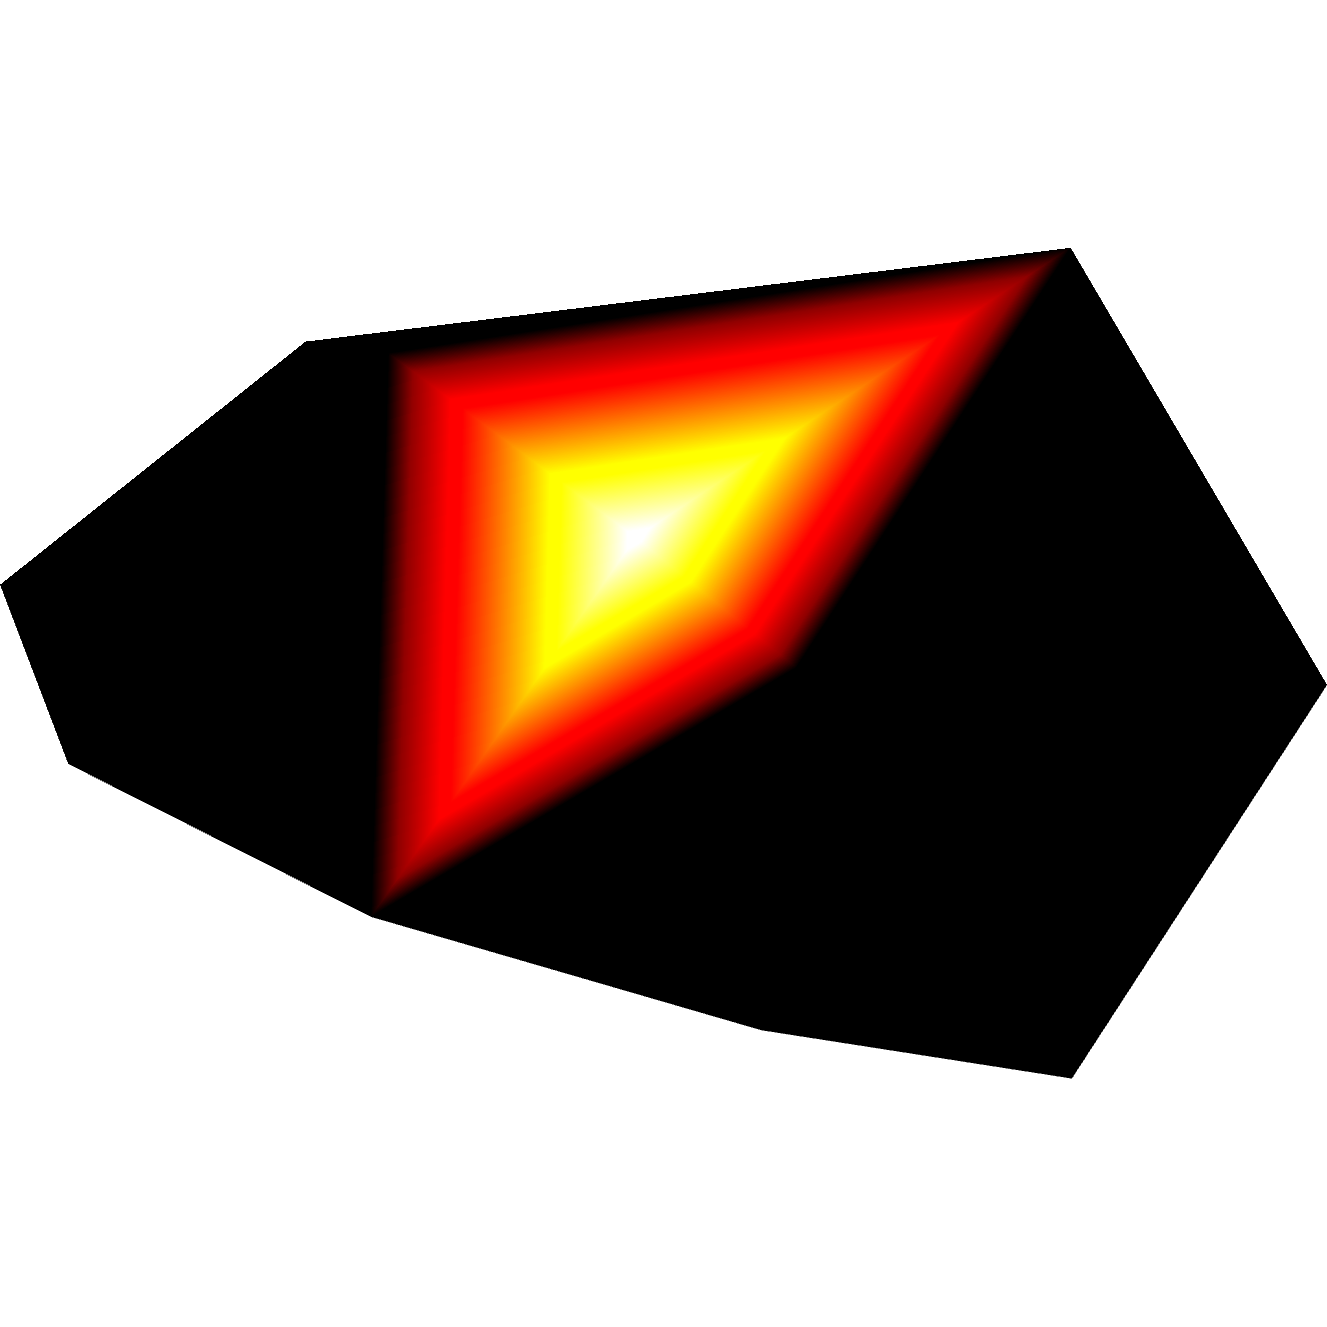
\includegraphics[width=1.0\linewidth,height=0.3\textheight,keepaspectratio,height=0.3\textheight,keepaspectratio]{data/synthetic_meshes/random_circle_tessellation_Dirac_delta_1_v11_f12_funcvals_0iter.png}
		\caption{R.Circ v11\_f12 iter 2}\label{fig:rcirc.e}
	\end{subfigure}
	\begin{subfigure}[b]{0.48\linewidth}
		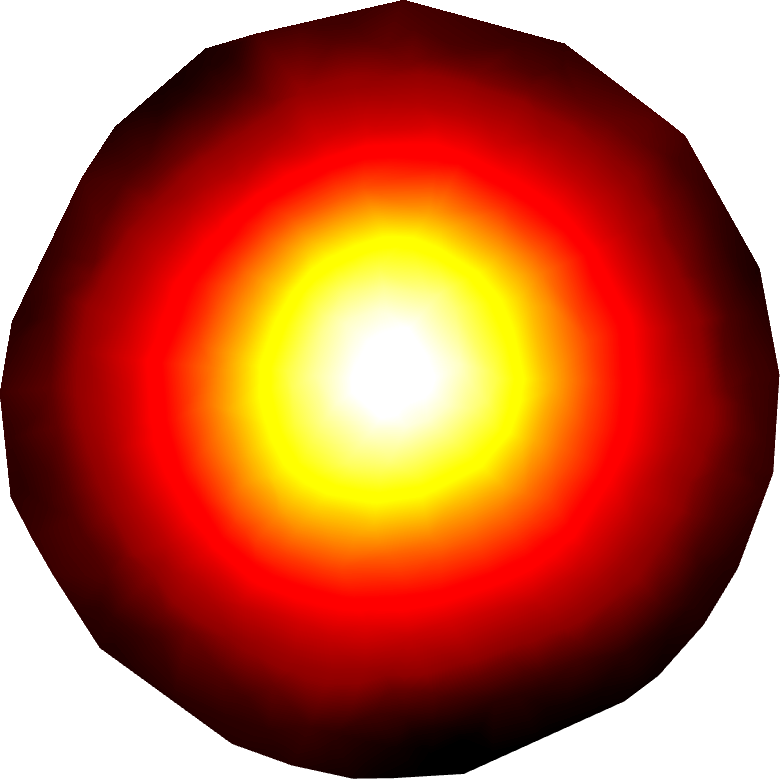
\includegraphics[width=1.0\linewidth,height=0.3\textheight,keepaspectratio,height=0.3\textheight,keepaspectratio]{data/synthetic_meshes/random_circle_tessellation_Dirac_delta_10_v641_f1252_funcvals_10000iter.png}
		\caption{R.Circ v641\_f1252 iter 10,000}\label{fig:rcirc.f}
	\end{subfigure}}
	{\caption[Synthetic random vertices equally distributed per radius, Dirac delta function]{A synthetic circle filled with random vertices equaly distributed per radius, triangulated by Delauney method~\cite[p.~??]{todoCitation}, with a Dirac delta function applied: (a) v11\_f12 wireframe (b) v641\_f1252 wireframe (c) v11\_f12 colored by function value before filter (d) v641\_f1252 colored by function value before filter (e) v11\_f12 colored by function value after 2 iterations (f) v641\_f1252 colored by function value after 10,000 iterations.
%All using the colorramp "Hot (improved)"~\cite[p.~???]{Brewer2003}~\cite[p.~19]{Giga17}, visualized using GigaMesh~\cite{Mara10}, exported as png after disabling the background grid [f7], maximizing the window, disabling screenshot cropping, as well as rejecting tiled rendering, finally cropping to content in GIMP.
}\label{fig:rcirc}}
\end{figure}
\todoCitation{}
\todoResearch{Why and who equally distributed}

